% define type of the document
\documentclass[a4paper,oneside,12pt]{article}
% set margins
\usepackage[margin=2.8cm]{geometry}
% set line width to 1.5
\usepackage{setspace}
\onehalfspacing
% use Times as de­fault text font and maths sup­port
\usepackage{mathptmx}

% set language to english, plus proper character encoding
\usepackage[utf8]{inputenc}
\usepackage[T1]{fontenc}
\usepackage[english]{babel}
% put quotations like # \enquote{quoted text} to get proper quotation marks
\usepackage[autostyle]{csquotes}

% enable colors
\usepackage{graphicx}
\usepackage{xcolor}
% hyperlinks in text, plus PDF with bookmarks
\usepackage{url}
\usepackage[hidelinks]{hyperref}
\usepackage{pdfpages}
%paragraphs and line spacing
%\setlength{\parindent}{0pt}
\usepackage{setspace}
\raggedbottom

% proper setting of units: # \unit[value]{unit} and chemical formulars # \ce{C2H4OH}
\usepackage[varioref=false,journal=angew]{chemstyle}
\usepackage[version=3]{mhchem}
\usepackage[loose,ugly]{units}

% enable nice tables
\usepackage{booktabs}
\usepackage{tabu}
\usepackage{multirow}

%bibliography options
\usepackage[backend=bibtex,defernumbers=true,natbib=true,style=numeric-comp,bibstyle=chem-angew,articletitle=true,sorting=none]{biblatex}
\addbibresource{references/references1.bib}



%header and footer
\usepackage{fancyhdr}
\pagestyle{fancy}
\renewcommand{\headrulewidth}{0pt}
\renewcommand{\footrulewidth}{1pt}
\lhead{}
\rhead{\thepage}
\cfoot{\textbf{Your Name Here} -- 6 Months Report, December, 2014}


% custom-made commands, e.g. \up{text} to easier set text superscript.
\newcommand{\up}[1]{\textsuperscript{#1}}
% use \scite[CitationKey] to set citations in [] and superscript
\newcommand{\scite}[1]{\textsuperscript{\cite{#1}}}
% use \sprime to set a proper prime character for nucleosides and nucleotides
\newcommand{\sprime}{\textsuperscript{$\prime$}}
% use \celsius to set °C properly
\newcommand{\degc}{$^{\circ}\mathrm{C}$}



% custom-made hypenation rules for words that might not occur in the dictionary of LaTeX
\hyphenation{de-ri-va-ti-za-tion}

% uncomment to enable title graphic (experimental)
%\usepackage[tc]{titlepic}
%\titlepic{\includegraphics[scale=1]{img_hi-logo.jpg}}


\begin{document}
\setstretch{1.2}

% set title page
\begin{titlepage}

\begin{center}
\huge{\textbf{A Short and Descriptive Title}}
\end{center}

\vspace{1cm}
\thispagestyle{empty}

\begin{center}
\textbf{Your Name Here}

\vspace{1cm}
 
\textbf{Sigurðsson Research Group \\
A 6 Month Progress Report \\
December 2014}
\end{center}

\vspace{10cm}

\begin{figure}[h!]
	\begin{center}
		
\includegraphics[scale=2]{figures/UIlogo}
	\end{center}
	\label{logo}
\end{figure}

\begin{center}
\textbf{University of Iceland \\
Department of Chemistry \\
Science Institute}
\end{center}

\end{titlepage}

% set table of contents
\tableofcontents

% include your texts
% Comment: The abstract will appear without a number, but will be listed in the table of contents.
\addcontentsline{toc}{section}{Abstract}
\section*{Abstract}

Write your abstract here.
\section*{Abbreviations}
\addcontentsline{toc}{section}{Abbreviations}

\begin{table}[h]
\begin{tabular}{ll}
DCM & dichloromethane\\
DMF & \emph{N},\,\emph{N}-dimethyformamide\\
DNA	&	deoxyribonucleic acid\\
EPR	& electron paramagnetic resonance\\
ESI-MS & electron-spray ionization mass-spectrometry\\
$J$ & coupling constant\\
$m/z$ & mass--charge ratio\\
NMR	& nuclear magnetic resonance\\
ppm & parts per million\\ 
RNA & ribonucleic acid\\
rt & room temperature (ambient)\\
TEA & triethylamine\\
THF & tetrahydrofurane\\
TFA & trifluoroacetic acid\\
TLC & thin layer chromatography\\
$\delta$	&	chemical shift\\
s & singlet\\
d	&	doublet\\
t	&	triplet\\
q	&	quartet\\
m	&	multiplet\\
\end{tabular}\hfill\
\end{table}

\section{Introduction}
Write your introduction here.

\begin{figure}[htb]
\begin{center}

\includegraphics[scale=0.7]{figures/image.png}
\caption{Caption text.}
\label{fig_sample-image}
\end{center}
\end{figure}

Figure  \ref{fig_sample-image} shows a sample image.
The DNA double helix was first reported by Watson and Crick in 1953.\cite{Watson1953} It also possible to put the citation in superscript, like this.\scite{Watson1953}
\section{Syntheses}
Write your syntheses here.

\begin{scheme}[ht]
\begin{center} 
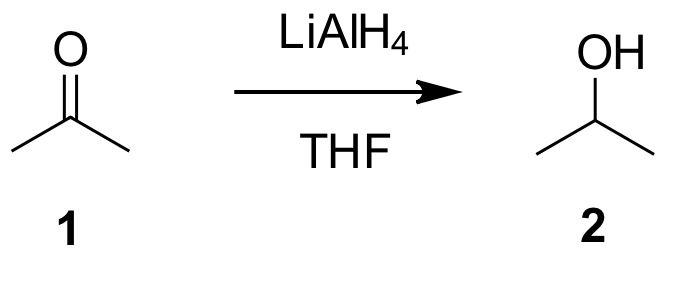
\includegraphics[scale=0.8]{schemes/scheme1.png}
\caption{A scheme with no compound numbers.}
\label{scheme_isoprop}
\end{center}
\end{scheme}

Scheme \ref{scheme_isoprop} shows a sample reaction scheme.
\section{Conclusions and Outlook}
Write your conclusions, and yout outlook here.

\section{Experiments}
\subsection{General}
Chemicals were purchased primarily from Sigma-Aldrich Chemical Company and Acros, Belgium, and were used without further purification.
Triethylamine was purchased anhydrous.
TLC was carried out using glass plates pre-coated with silica gel (F254, Silicycle SiliPlate 60~\AA ). 
Visualisation was by UV light, and \ce{I2} staining, respectively.
Silica gel was purchased from Silicycle, and used for medium pressure chromatography (\enquote{flash}-chromatography).

\up{1}H and \up{13}C NMR spectra were recorded at the frequencies stated, using deuterated chloroform as internal standard ($\delta$ = 7.26~ppm for \up{1}H and $\delta$ = 77.0~ppm for \up{13}C NMR).
400 MHz spectra were recorded on a Bruker Advance 400 spectrometer.
All coupling constants were measured in Hertz.

All moisture sensitive reactions were carried out in flame-dried glassware using argon from standard BOC industrial cylinders, dried through an activated silica column. Diethyl ether for moisture-sensitive reactions was used freshly distilled over Na under argon atmosphere.
Concentrations of \nBu Li in hexane were determined by titration using diphenylacetic acid.

\newpage
\subsection{1,2,4,5-Tetra-\textit{tert.}-butyl\-thio\-benzene~(\textbf{1})}

\begin{scheme}[ht]
\begin{center} 
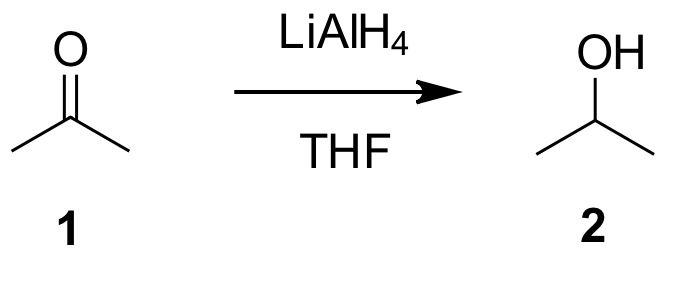
\includegraphics[scale=0.8]{schemes/scheme1.png}
\end{center}
\end{scheme}

To a solution of 2-methyl-2-propanethiol (94~mL, 0.84~mol) in DMF (150~mL) was added small pieces of sodium (19.37~g, 0.84~mol) at 0~\degc. The mixture was allowed to reach ambient temperature and was stirred overnight. 1,2,4,5-Tetrachlorobenzene (30.3~g, 140.6~mmol) was added at once, and the resulting mixture was heated to 90~\degc.
As soon as the reaction mixture darkened and steam started to develop, the heating source was removed.
As soon as the exothermic reaction had finished, the mixture was heated to 120~\degc for 24~h. 
After being cooled to ambient temperature, the reaction mixture was poured over ice. The precipitate was removed by filtration, washed with water, and dried to give 30~g (49.5\%) of the product as an off-white powder.\\

\noindent
Notebook reference: MKI-107.\\

\noindent
\up{1}H~NMR (400MHz, \ce{CDCl3}) $\delta$ = 7.94 (2 H, s),1.36 ppm (2 H, s).\\

\noindent
\up{13}C~NMR (101 MHz, \ce{CDCl3}) $\delta$ = 144.78, 139.36, 48.13, 31.33 ppm.


% set bibliography and add to table of contents, but without numbering
\newpage
\phantomsection \label{bibliography}
\addcontentsline{toc}{section}{Bibliography}
\printbibliography[resetnumbers=true]

% same goes for the list of figures
\newpage
\phantomsection \label{listoffig}
\addcontentsline{toc}{section}{List of Figures}
\listoffigures

\newpage
\phantomsection \label{listofschemes}
\addcontentsline{toc}{section}{List of Schemes}
\listofschemes

% uncomment to allow list of tables
%\newpage
%\phantomsection \label{listoftabs}
%\addcontentsline{toc}{chapter}{List of Tables}
%\listoftables

\end{document}